\section{Ford Fulkerson}

\subsection{Sequential Algorithm}
    Ford-Fulkerson (FF) is a greedy algorithm to get the maximum flow of a graph.  The typical implementation of FF is through using Depth First Search (DFS). The other algorithms described in the other sections are variations based off of FF; however, the goal of this section of the project seeks to parallelize the traditional DFS approach \cite{FFvEk} of FF as other implementations such as Edmond Karp or Dinics takes advantage of specific graph structures.
    \newline
    
    \subsubsection{Pseudo Code of Sequential}
    Note if there are $n$ nodes, each node will be indexed from 0 through $n-1$. In the algorithm, the Source node is indexed as 0 while the Sink node is indexed as $n-1$
    \begin{algorithmic}
        \State Node:
            \State $prevNode \gets$ Integer
            \State $thisNode \gets$ Integer
            \State $add \gets$ Boolean
            \State $potentialFlow \gets$ Integer\\
            
        
        \State FordFulkerson:
            \State $capacity[][] \gets$ Capacity Graph
            \State $flow[][] \gets$ Flow Graph
            \State $nodeLabels \gets$ Array of Nodes
            \State $numNodes \gets$ Number of nodes in graph\\
            \State $sink \gets$ Integer\\
            
            \For {i in range 2:}
                \For {i in range numNodes:}
                    \For {j in range numNodes:}
                        \If {jth-node is labeled}
                            \State
                                \If {ith-node is not labeled and $flow[j][i] < cap[j][i]$}
                                    Label() where $add$ is true
                                \EndIf
                                
                                \If {ith-node is not labeled and $flow[j][i] >$ 0}
                                    Label() where $add$ is false
                                \EndIf
                        \EndIf
                    \EndFor
                    
                    \If{sink node is labeled}
                        Augment()
                        then do outermost for-loop again
                    \EndIf
                \EndFor
            \EndFor\\
            
            End algorithm\\\\

        \Function{augment}{}
            \State $tN \gets sink node$ 
            \State $augNum \gets Integer$ 
        
            \While {$tN$ is not 0}
                \If{$tN.thisNode$}
                    \State $flow[tN.prevNode][tN.thisNode] \gets$ flow[tN.prevNode][tN.thisNode] + augNum
                
                \Else \State $flow[tN.thisNode][tN.prevNode] \gets$ flow[tN.thisNode][tN.prevNode] - augNum
                    
                \EndIf
                
                \State $tN \gets tN$'s previous node
            \EndWhile
        \EndFunction\\\\

        \Function{label}{}
            \If {$add:$}
            	\State 
            	    $pFlow \gets$ min(ith-node's potentialFlow, cap[i][j] - flow[i][j])
            \Else
                \State
			        $pFlow \gets$ min(ith-node's potentialFlow, flow[j][i])
            \EndIf
        \EndFunction
    \end{algorithmic}
\subsection{Parallel Algorithm}
    \subsubsection{Research}
        The approach used in a parallel algorithm of Ford-Fulkerson already posed intimidating challenges. Unlike its sibling algorithms, Edmond-Karp in particular, FF is traditionally implemented using DFS, not breadth-first-search (BFS). Without the luxury of a an easily-parallelizable algorithm, research had to be done to convert a recursive DFS approach into an iterative one.
        
        During a run of FF, the algorithm attempts to find augmenting paths by conducting two primary steps: searching for a valid flow-augmenting path, and then proceeding to update the flow-augmenting paths on a backward pass.
        
        
    \subsubsection{Algorithmic Approach}
        Three options of parallelization were considered during the process of Ford-Fulkerson:
        \begin{enumerate}
            \item Depth-First Search
            \item Augmenting Paths
            \item Backwards Update
        \end{enumerate}
        Attempting to create an iterative version of DFS would have involved the usage of additional overhead in order to simulate recursion, such as the introduction of a stack.
        
        Rather than navigating through the difficulties of directly turning DFS parallel, a hybrid solution was attempted, where the process of traversing a graph's adjacency matrix was combined with labeling the current flow running through the network flow graph. In the end the attempted solution combines the greedy approach from augmenting the paths by overlapping threads across different connected edges.
        
        
    \subsubsection{Initial Approach}
        The adjacency matrix used to represent the flow and the capacity could be parsed in two different ways. Instead of utilizing a traditional row $\xrightarrow{}$ column approach to navigate through the matrix, instead a column $\xrightarrow{}$ row method will be chosen in order to avoid overhead issues that could arise with multiple threads.
        The Initial Approach is the same as the Final Approach below with the exception of the direction of "sweeping" when labeling a node. In the Initial Approach, threads would sweep from left-to-right in the capacity matrix column-by-column. Unfortunately, this particular method of labeling the nodes raises contention issues in the form of multiple threads attempting to acquire a lock if for example: we were labeling the flow from node S to A.
        
        
    \subsubsection{Final Approach}
        The chosen parallel approach allows multiple threads to search through the graph's adjacency matrix and interdependently adjust potential flow as all threads traverse the matrix together column-by-columns.
        
        In the Final Approach, threads would sweep from top-to-bottom in the capacity matrix. This is an improvement compared to the Initial Approach 
        since there will be no contention when it comes to labeling a node. This occurs since each thread will attempt to assign a label to a different node.
        
        The method of labeling was discovered independent of existing research papers while tracing through multiple scenarios of multiple threads attempting to augment the graph. An important conclusion was that when augmenting a path, a single thread must complete this without interruption. This means once a thread reaches the sink node, it locks the other threads from augmenting.
    
    \subsubsection{Tracing Through The Final Approach}
        \begin{figure}[H]
            \centering
            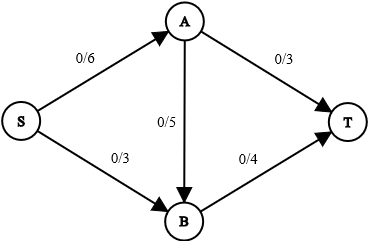
\includegraphics[scale=0.80]{figures/graph.png}
            \caption{Network Flow Graph}
        \end{figure}
    
        \begin{figure}[H]
            \centering
            \[
                \begin{blockarray}{ccccc}
                    & S & A & B & T \\
                    \begin{block}{c(cccc)}
                        S & 0 & 6 & 3 & 0 \\
                        A & 0 & 0 & 5 & 3 \\
                        B & 0 & 0 & 0 & 4 \\
                        T & 0 & 0 & 0 & 0 \\
                    \end{block}
                \end{blockarray}
            \]
            \caption{Adjacency Matrix of Fig. 1's capacity}
        \end{figure}
        
        \begin{figure}[H]
            \centering
            \[
                \begin{blockarray}{ccccc}
                    & S & A & B & T \\
                    \begin{block}{c(cccc)}
                        S & 0 & 0 & 0 & 0 \\
                        A & 0 & 0 & 0 & 0 \\
                        B & 0 & 0 & 0 & 0 \\
                        T & 0 & 0 & 0 & 0 \\
                    \end{block}
                \end{blockarray}
            \]
            \caption{Starting Adjacency Matrix of Fig. 1's flow}
        \end{figure}
        
        Figure 1 and 2 will be used as an example to illustrate how the parallel approach works. There is also another adjacency matrix of the same size as the capacity matrix which keeps track of the flow after augmenting a graph. This flow matrix has a starting state where all the values are initialized to 0. The notation flow[0][1] means get the element on the 0th row and 1st column of the flow matrix. The notation cap[0][1] means get the element on the 0th row and 1st column of the capacity matrix (this would be 6 on Figure 2).
        
        
        
        $S$ is the Source node and $T$ is the Sink node. Assume the use of 2 threads X and Y. The notation of X:cap[1][2] means thread X is looking at the capacity of 5. Begin all threads in the 0th-index row ($S$).
        
        
        Initially, the threads will be at X:cap[0][1] and Y:cap[0][2] (Note that the Source node column (cap[\_][0]) can be skipped since there are no incoming edges to the source node. So the threads can be X:cap[0][0] and Y:cap[0][1] but it is not done here in the example as it is not as helpful for demonstration nor is it efficient). The two threads will then sweep through the rows from top-to-bottom in order to label nodes.
        
        A label will be in the form of a tuple (Ex. (A, +, 6)) which describe, respectively, what node it came from, what operation (add or subtract) to do when augmenting, and the potential flow of the labeled node. Some things to note is that the Source node is always labeled as (\_, +, $\infty$); once the Sink node is labeled, start the augmentation of the graph by backtracking through the labels of the nodes and use the potential flow labeled on the Sink node when augmenting each of the edges. \newline
        
        We only label a node if it is not already labeled and:
        \begin{enumerate}
            \item (Forward Edge) The flow of the edge from previous node (prev) to current node (curr) is less than the capacity from prev to curr.\newline
            For i, j, where they are the index of the prev node and curr node respectively, $flow[i][j] < cap[i][j]$. This would result in a labeling of (prev, +, min\{prevPotentialFlow, cap[i][j] - flow[i][j]\}). prevPotentialFlow is simply the third item of the tuple in the label of the previous node.
            \item (Backward Edge) The flow of the edge from the curr node to the prev node is greater than 0.\newline
            For i, j, where they are the index of the prev node and curr node respectively, $flow[j][i] > 0$. This would result in a labeling of (prev, -, min\{prevPotentialFlow, flow[j][i]\})\newline
        \end{enumerate}
        
        Using the rules above, for thread X currently at X:cap[0][1], X will label node $A$ because the previous node $S$ is labeled (with (\_, +, $\infty$)) and $X:flow[0][1] < X:cap[0][1]$. With this, node $A$ will be labeled with (S, +, 6). For thread Y currently at Y:cap[0][2], Y will label node $B$ because the previous node $S$ is labeled and $Y:flow[0][1] < Y:cap[0][2]$. Hence, node $B$ will be labeled with (S, +, 3). The graph and matrix are shown below.
        
        
        
        \begin{figure}[H]
            \centering
            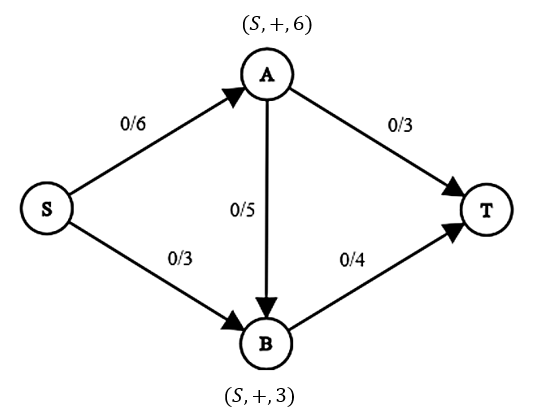
\includegraphics[scale=.5]{figures/nodeAandB.png}
            \caption{Threads X and Y simultaneously labeling nodes A and B.}
            \label{fig:Sweep}
        \end{figure}
        \begin{figure}[H]
            \centering
            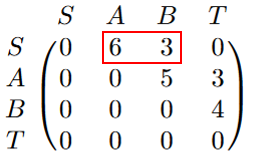
\includegraphics[scale=.5]{figures/Sweep.png}
            \caption{X:cap[0][1] and Y:cap[0][2] on an initial sweep}
            \label{fig:Sweep}
        \end{figure}
        
        After the two threads in this example finished labeling in the 0th-index row, both threads move to the 1st-index row in the same respective column. So X:cap[1][1] and Y:cap[1][2] are the next elements the threads will attempt to label. It will be found that X any Y will not label $A$ and $B$ since $A$ and $B$ was already labeled in the previous iteration.
        Hence, the graph in this iteration will look the same as Figure 4.
        
        \begin{figure}[H]
            \centering
            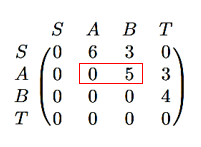
\includegraphics[scale=.7]{figures/Sweep2.png}
            \caption{X:cap[1][1] and Y:cap[1][2] on next sweep}
            \label{fig:Sweep}
        \end{figure}
        
        The threads will continue to sweep down. When it reaches the last row, the threads shift over right 1 column and goes back to the 0th-index to do another top-to-bottom sweep. If the threads shift over past the number of columns, it cycles back to the 0th-index column and continues.

        \begin{figure}[H]
            \centering
            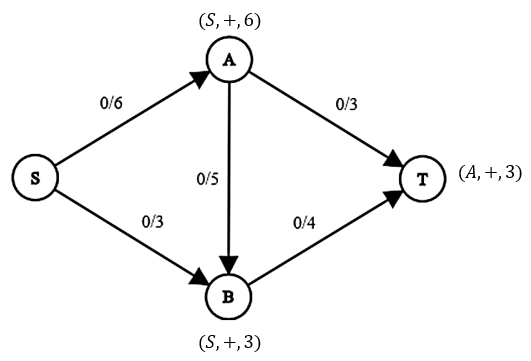
\includegraphics[scale=.6]{figures/hitsink.png}
            \caption{Labeling sink}
            \label{fig:Sweep}
        \end{figure}
        
        \begin{figure}[H]
            \centering
            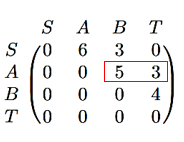
\includegraphics[scale=.7]{figures/cap[1][3].png}
            \caption{X:cap[1][1] and Y:cap[1][2] on sweep}
            \label{fig:Sweep}
        \end{figure}
        
        After some amount of sweeps, the threads go to the 1st-index row (A) with X:cap[1][2] and Y:cap[1][3]. Y:cap[1][3] will label the Sink node with (A, +, 3). Since Sink is labeled, augment the graph by backtracking through the labels and use the potential flow of the Sink node label, which is 3, on all the edges. Add or subtract that potential flow based on the 2nd item in the tuple of the label that is currently being scanned. The augmenting ends once the Source node is reached. This was the first augmentation of many that will occur in the graph. Below is the first augmented graph of many.
        
        \begin{figure}[H]
            \centering
            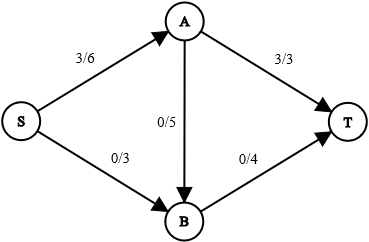
\includegraphics[scale=.7]{figures/FFaugmented.png}
            \caption{The graph after augmenting}
            \label{fig:Sweep}
        \end{figure}
        
        The algorithm continues augmenting the graph until an iteration cannot label any nodes after a top-to-bottom sweep. When the algorithm ends, the maximum flow is found by finding the sum of the flow column of the sink node.
        
        \begin{figure}[H]
            \centering
            \[
                \begin{blockarray}{ccccc}
                    & S & A & B & T \\
                    \begin{block}{c(cccc)}
                        S & 0 & 4 & 3 & 0 \\
                        A & 0 & 0 & 1 & 3 \\
                        B & 0 & 0 & 0 & 4 \\
                        T & 0 & 0 & 0 & 0 \\
                    \end{block}
                \end{blockarray}
            \]
            \caption{Adjacency Matrix of flow after finished algorithm}
        \end{figure}
        
        Hence, the max flow of the graph in this example is 7.
        
    \subsubsection{Pseudo Code of Parallel}
        Note if there are $n$ nodes, each node will be indexed from 0 through $n-1$. In the algorithm, the Source node is indexed as 0 while the Sink node is indexed as $n-1$
        \begin{algorithmic}
            \State Node:
                \State $prevNode \gets$ Integer
                \State $thisNode \gets$ Integer
                \State $add \gets$ Boolean
                \State $potentialFlow \gets$ Integer\\
                
            \State FordFulkerson:
                \State $row \gets$ AtomicInteger
                \State $capacity[][] \gets$ Capacity Graph
                \State $flow[][] \gets$ Flow Graph
                \State $nodeLabels[] \gets$ Array of Nodes
                \State $numNodes \gets$ number of nodes in graph
                \State $threadLimit \gets$ Max number of threads
                \State $tNum \gets$ Identifying Thread number 0-indexed
                \\
                
                \For {offset in range numNodes:}
                    \State i $\gets$ ((offset * threadLimit) + tNum) \% numNodes
                    \For {$row$ in range numNodes:}
                        \State j $\gets row$
                        \If {jth-node is labeled}
                            \State
                                \If {ith-node is not labeled and $flow[j][i] < cap[j][i]$}
                                    Label() where $add$ is true
                                \EndIf
                                
                                \If {ith-node is not labeled and $flow[j][i] >$ 0}
                                    Label() where $add$ is false
                                \EndIf
                        \EndIf\\
                        waitForAllThreadsBeforeProceeding()
                    \EndFor
                    \If{sink node is labeled}
                        Only one thread Augment()\\
                        waitForAllThreadsBeforeProceeding()\\
                        do outermost for-loop again
                    \EndIf\\
                \EndFor\\
                
                End algorithm\\\\
                
            \Function{augment}{}
                \State $tN \gets sink node$ 
                \State $augNum \gets Integer$ 
            
                \While {$tN$ is not 0}
                    \If{$tN.thisNode$}
                        \State $flow[tN.prevNode][tN.thisNode] \gets$ flow[tN.prevNode][tN.thisNode] + augNum
                    
                    \Else \State $flow[tN.thisNode][tN.prevNode] \gets$ flow[tN.thisNode][tN.prevNode] - augNum
                        
                    \EndIf
                    
                    \State $tN \gets tN$'s previous node
                \EndWhile
            \EndFunction\\\\
    
            \Function{label}{}
                \If {$add:$}
                	\State 
                	    $pFlow \gets$ min(ith-node's potentialFlow, cap[i][j] - flow[i][j])
                \Else
                    \State
    			        $pFlow \gets$ min(ith-node's potentialFlow, flow[j][i])
                \EndIf
            \EndFunction
            \end{algorithmic}\\

\subsection{Testing \& Result}
    These test results were performed on UCF's Eustis3 server utilizing open-source datasets \cite{sumitpadhiyar}
    \begin{tabular}{ | m{4em} | m{5em }| m{5em} | m{5em} | } 
      \hline
      Nodes & Max Flow & Sequential Time & Parallel Time \\ 
      
        \hline
        50      & 828     & 5ms &\\
        \hline
        100     & 1251    & 10ms & \\  
        \hline
        500     & 7143    & 182ms & \\        
        \hline   
        750     & 10930   & 396ms & \\         
        \hline
        1000    & 13476   & 866ms & \\       
        \hline
        2000    & 25027   & 6532ms & \\
        \hline
        3000    & 39170   & 18448ms & \\       
        \hline
        4000    & 58517   & 53893ms & \\
        \hline
        5000    & 69349   & 117045ms & \\
        \hline
        10000   & 142610  & 784219ms & \\
        \hline
    \end{tabular}